\documentclass[aspectratio=169,utf8,t]{beamer}

% Idioma e Codificacao
\usepackage[brazilian]{babel}
\usepackage{booktabs}
\usepackage{array}
\usepackage{listings}
\usepackage{amsmath}
\usepackage{amssymb}
\usepackage{graphicx}

% Carrega o Tema Modelo dos Scouts (Widescreen 16:9, Nunito Sans)
\usetheme{scouts}

% Configuracao para Codigo-Fonte (Bash / Python / Redis)
\lstset{
    basicstyle=\fontsize{6.5pt}{8.2pt}\selectfont\ttfamily,
    keywordstyle=\bfseries\color{ScoutNavy},
    stringstyle=\color{ScoutGreen},
    commentstyle=\itshape\color{gray},
    backgroundcolor=\color{black!3},
    frame=single,
    rulecolor=\color{black!15},
    breaklines=true,
    breakatwhitespace=true,
    showstringspaces=false,
    tabsize=2,
    aboveskip=4pt,
    belowskip=3pt
}

% Metadados Institucionais
\author{Prof. Me. Reginaldo Fernandes}
\institute{Instituto Federal do Ceará -- Campus Tauá \\ Tecnologia em Análise e Desenvolvimento de Sistemas}
\title{Bancos de Dados Não-Relacionais}
\subtitle{Aula 04: Modelo Chave-Valor, Arquitetura em Memória e Estruturas Nativas do Redis}
\date{13 de Outubro de 2026}

\begin{document}

% ------------------------------------------------------------------------------
% Capa da Apresentacao
% ------------------------------------------------------------------------------
\changecolours[inverse]{ScoutGreen}
\frame[plain]{\titlepage}

% ------------------------------------------------------------------------------
% Sumario Executivo da Aula
% ------------------------------------------------------------------------------
\changecolours{ScoutGreen}
\begin{frame}{Agenda do Encontro}
  \vspace{0.4cm}
  \tableofcontents
\end{frame}

% ------------------------------------------------------------------------------
% Modulos da Aula
% ------------------------------------------------------------------------------
\changecolours{ScoutNavy}
\section{O Modelo Chave-Valor e o Ecossistema Redis}

% ------------------------------------------------------------------------------
\twocolframe[title={O Paradigma Chave-Valor (Key-Value)},leftcol=7cm,rightcol=7cm]{%
  \alert{Simplicidade e Desempenho Extremo}\par
  \itemseps[topsepi=2mm,itemsepi=3mm,labelsep=2mm,leftmargini=4mm]
  \begin{itemize}
    \item Entre os 4 modelos NoSQL, o \textbf{Chave-Valor} é o mais primitivo e veloz.
    \item Cada dado é indexado por uma única chave opaca (\textit{Key}).
    \item O valor associado (\textit{Value}) é tratado como uma carga útil (\textit{payload}).
    \item \textbf{Complexidade de Busca:} Tempo constante $\mathcal{O}(1)$ via tabela hash interna.
  \end{itemize}
}{%
  \alert{Por que o Redis se Destaca no Mercado?}\par
  \itemseps[topsepi=2mm,itemsepi=3mm,labelsep=2mm,leftmargini=4mm]
  \begin{itemize}
    \item Criado por \textbf{Salvatore Sanfilippo (antirez)} em 2009.
    \item Sigla: \textbf{REmote DIctionary Server}.
    \item \textbf{In-Memory Engine:} Opera 100\% na memória RAM com latência sub-milissegundo ($< 1$ ms).
    \item Não armazena apenas strings brutas, mas \textbf{estruturas de dados ricas}.
  \end{itemize}
}

% ------------------------------------------------------------------------------
\twocolframe[title={Ambiente Windows: Por que Usar o WSL 2?},leftcol=7cm,rightcol=7cm]{%
  \alert{Natureza POSIX do Redis}\par
  \itemseps[topsepi=2mm,itemsepi=3mm,labelsep=2mm,leftmargini=4mm]
  \begin{itemize}
    \item O Redis depende de primitivas POSIX (Linux/Unix), como \texttt{fork()} para persistência em segundo plano.
    \item Não há binário oficial para Windows nativo desde a versão 3.2.
    \item Versões não-oficiais para Windows apresentam instabilidade e faltam recursos modernos.
  \end{itemize}
}{%
  \alert{A Solução Definitiva: WSL 2}\par
  \itemseps[topsepi=2mm,itemsepi=3mm,labelsep=2mm,leftmargini=4mm]
  \begin{itemize}
    \item O \textbf{Windows Subsystem for Linux 2} roda um kernel Linux real sobre hipervisor leve.
    \item \textbf{Desempenho Idêntico ao Linux:} Sem degradação em chamadas de sistema.
    \item \textbf{Rede Transparente:} O Windows mapeia \texttt{localhost:6379} automaticamente para IDEs e Python.
  \end{itemize}
}

% ------------------------------------------------------------------------------
\begin{frame}[fragile]{Instalação e Execução do Redis no WSL 2}
  \begin{columns}[T]
    \begin{column}{0.48\textwidth}
      \alert{1. Instalação do Ambiente Linux}\par
      \itemseps[topsepi=1mm,itemsepi=1.5mm,labelsep=2mm,leftmargini=4mm]
      \begin{itemize}
        \item No PowerShell (Administrador):
      \end{itemize}
      \begin{lstlisting}[language=bash]
# Instala o Ubuntu no WSL 2:
wsl --install -d Ubuntu
      \end{lstlisting}
      \vspace{0.1cm}
      \alert{2. Pacote Oficial no Ubuntu}\par
      \begin{lstlisting}[language=bash]
# Atualiza repositorios e instala:
sudo apt update
sudo apt install redis-server -y
      \end{lstlisting}
    \end{column}
    \begin{column}{0.50\textwidth}
      \alert{3. Gerenciamento do Serviço}\par
      \begin{lstlisting}[language=bash]
# Iniciar o servidor Redis:
sudo service redis-server start

# Verificar se esta rodando:
sudo service redis-server status
      \end{lstlisting}
      \vspace{0.1cm}
      \alert{4. Teste de Conexão}\par
      \begin{lstlisting}[language=bash]
# Abrir console interativo:
redis-cli
127.0.0.1:6379> PING
PONG
      \end{lstlisting}
    \end{column}
  \end{columns}
\end{frame}

% ------------------------------------------------------------------------------
\begin{frame}[fragile]{Convenção de Chaves e Diagnóstico no redis-cli}
  \begin{columns}[T]
    \begin{column}{0.48\textwidth}
      \alert{Convenção de Namespaces}\par
      \itemseps[topsepi=1mm,itemsepi=1.5mm,labelsep=2mm,leftmargini=4mm]
      \small
      \begin{itemize}
        \item O Redis não possui schemas relacionais.
        \item Chaves são organizadas com dois-pontos (\texttt{:}):
        \item \textbf{Padrão:} \texttt{\scriptsize modulo:entidade:id:campo}
        \item \textbf{Exemplo:} \texttt{\scriptsize loja:prod:42:preco}
        \item Garante legibilidade e isolamento.
      \end{itemize}
    \end{column}
    \begin{column}{0.50\textwidth}
      \alert{Diagnóstico no redis-cli}\par
      \begin{lstlisting}[language=bash]
# Testar eco e latencia:
127.0.0.1:6379> PING "IFCE Taua"
"IFCE Taua"

# Diagnostico do servidor:
127.0.0.1:6379> INFO server
# Retorna versao, PID e uptime

# Contagem total de chaves:
127.0.0.1:6379> DBSIZE
(integer) 42
      \end{lstlisting}
    \end{column}
  \end{columns}
\end{frame}

\changecolours{ScoutGreen}
\section{Arquitetura em Memória e Mecanismos de Persistência}

% ------------------------------------------------------------------------------
\twocolframe[title={A Memória RAM: Velocidade Extrema vs Volatilidade},leftcol=7cm,rightcol=7cm]{%
  \alert{Por que o Redis é Tão Rápido?}\par
  \itemseps[topsepi=2mm,itemsepi=3mm,labelsep=2mm,leftmargini=4mm]
  \begin{itemize}
    \item Acesso direto à memória RAM sem overhead de barramento mecânico ou NVMe.
    \item Latência típica: \textbf{70 microssegundos} ($\approx 0,07$ ms).
    \item \textbf{O Dilema Físico:} A memória RAM é \textbf{volátil}. Se o servidor reiniciar ou faltar energia, todos os dados são apagados.
  \end{itemize}
}{%
  \alert{A Solução: Persistência em Disco}\par
  \itemseps[topsepi=2mm,itemsepi=3mm,labelsep=2mm,leftmargini=4mm]
  \begin{itemize}
    \item O Redis não é apenas um cache efêmero; ele pode operar como banco de dados durável.
    \item O motor oferece dois mecanismos nativos de armazenamento não-volátil:
    \item \textbf{1. RDB (Snapshotting):} Fotografias pontuais em disco.
    \item \textbf{2. AOF (Append-Only File):} Diário contínuo de operações.
  \end{itemize}
}

% ------------------------------------------------------------------------------
\begin{frame}{Arquitetura em Memória vs Armazenamento Persistente}
  \centering
  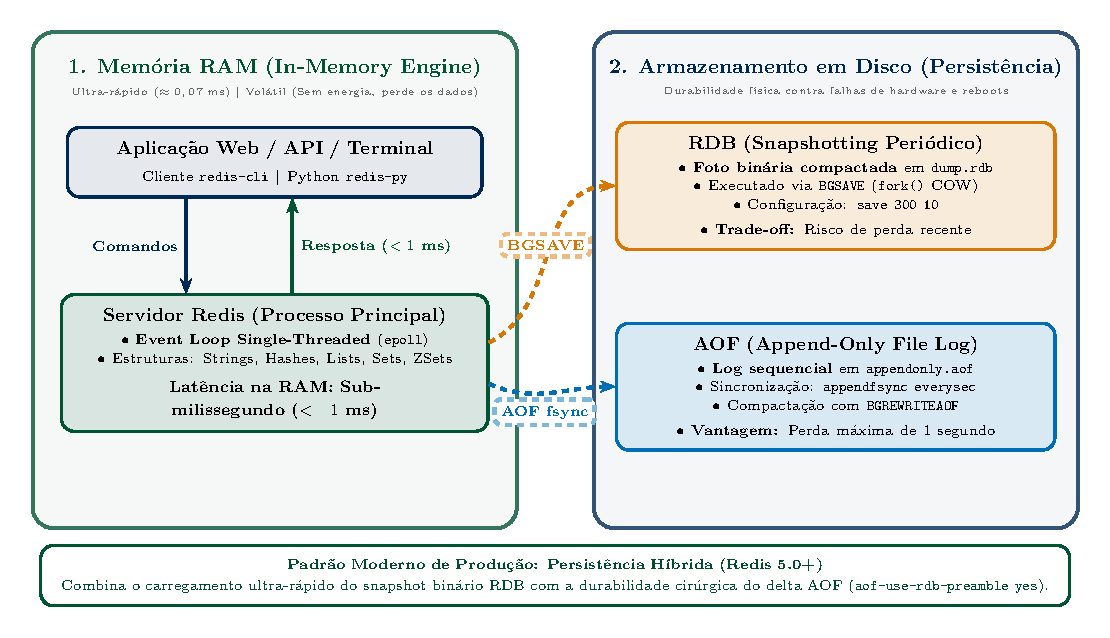
\includegraphics[width=0.90\textwidth,height=0.74\textheight,keepaspectratio]{figuras/fig_arquitetura_memoria_persistencia.pdf}
\end{frame}

% ------------------------------------------------------------------------------
\twocolframe[title={Mecanismo 1: RDB (Snapshotting e BGSAVE)},leftcol=7cm,rightcol=7cm]{%
  \alert{Como Funciona o Snapshotting}\par
  \itemseps[topsepi=2mm,itemsepi=3mm,labelsep=2mm,leftmargini=4mm]
  \begin{itemize}
    \item O RDB grava uma cópia binária compactada de toda a memória no arquivo \texttt{dump.rdb}.
    \item Ideal para \textbf{backups periódicos} e recuperação de desastres.
    \item \textbf{Ponto de Restauração:} Se houver falha, dados gerados após o último snapshot são perdidos.
  \end{itemize}
}{%
  \alert{Diferença Crítica: BGSAVE vs SAVE}\par
  \itemseps[topsepi=2mm,itemsepi=3mm,labelsep=2mm,leftmargini=4mm]
  \begin{itemize}
    \item \textbf{SAVE (Síncrono / Bloqueante):} Trava a thread do Redis. Nenhuma consulta é respondida até terminar. \textbf{Nunca use em produção!}
    \item \textbf{BGSAVE (Assíncrono / Não-bloqueante):} Dispara processo filho via \texttt{fork()} com \textit{Copy-on-Write} (COW). Atende conexões sem interrupção.
  \end{itemize}
}

% ------------------------------------------------------------------------------
\begin{frame}[fragile]{Configuração do RDB e Comandos no redis-cli}
  \begin{columns}[T]
    \begin{column}{0.48\textwidth}
      \alert{Regras de Disparo no redis.conf}\par
      \begin{lstlisting}[language=bash]
# Sintaxe: save <segundos> <alteracoes>
save 900 1      # 15 min se 1 chave mudou
save 300 10     # 5 min se 10 chaves mudaram
save 60 10000   # 1 min se 10k chaves mudaram

# Destino do snapshot binario
dbfilename dump.rdb
dir /var/lib/redis
      \end{lstlisting}
    \end{column}
    \begin{column}{0.50\textwidth}
      \alert{Disparo Manual via redis-cli}\par
      \begin{lstlisting}[language=bash]
# Disparar snapshot assincrono:
127.0.0.1:6379> BGSAVE
Background saving started

# Timestamp UNIX do ultimo dump:
127.0.0.1:6379> LASTSAVE
(integer) 1791888929

# Inspecionar status de persistencia:
127.0.0.1:6379> INFO persistence
# rdb_last_bgsave_status:ok
      \end{lstlisting}
    \end{column}
  \end{columns}
\end{frame}

% ------------------------------------------------------------------------------
\twocolframe[title={Mecanismo 2: AOF (Append-Only File)},leftcol=7cm,rightcol=7cm]{%
  \alert{Diário Sequencial de Operações}\par
  \itemseps[topsepi=2mm,itemsepi=3mm,labelsep=2mm,leftmargini=4mm]
  \begin{itemize}
    \item Registra cada comando de escrita recebido em modo append (\texttt{appendonly.aof}).
    \item Na reinicialização, o Redis reproduz o diário para reconstruir o estado com quase zero perda.
    \item \textbf{BGREWRITEAOF:} Compacta o diário em background removendo comandos obsoletos.
  \end{itemize}
}{%
  \alert{Políticas de Sincronização (fsync)}\par
  \itemseps[topsepi=2mm,itemsepi=3mm,labelsep=2mm,leftmargini=4mm]
  \begin{itemize}
    \item \textbf{appendfsync always:} Sincroniza a cada comando. Durabilidade máxima, menor vazão.
    \item \textbf{appendfsync everysec (Padrão Recomendado):} Descarrega em disco a cada 1 segundo. Máxima perda: 1 segundo de dados.
    \item \textbf{appendfsync no:} O SO decide quando gravar.
  \end{itemize}
}

% ------------------------------------------------------------------------------
\begin{frame}[fragile]{Configuração do AOF e Persistência Híbrida}
  \begin{columns}[T]
    \begin{column}{0.48\textwidth}
      \alert{Diretivas no redis.conf}\par
      \begin{lstlisting}[language=bash]
# Habilitar o modo Append-Only
appendonly yes
appendfilename "appendonly.aof"

# Frequencia de flush fsync em disco
appendfsync everysec

# Persistencia Hibrida (Padrao Redis 5+)
# Salva RDB no inicio + AOF no final
aof-use-rdb-preamble yes
      \end{lstlisting}
    \end{column}
    \begin{column}{0.50\textwidth}
      \alert{Compactação e Inspecção no CLI}\par
      \begin{lstlisting}[language=bash]
# Reescrever diario AOF em background:
127.0.0.1:6379> BGREWRITEAOF
Background append only file rewriting started

# Consultar estatisticas detalhadas:
127.0.0.1:6379> INFO persistence
# aof_enabled:1
# aof_rewrite_in_progress:0
      \end{lstlisting}
    \end{column}
  \end{columns}
\end{frame}

\changecolours{ScoutNavy}
\section{Variações Avançadas dos Comandos SET e GET}

% ------------------------------------------------------------------------------
\twocolframe[title={Problema Real Inicial: Cache de Termos de Busca},leftcol=7cm,rightcol=7cm]{%
  \alert{O Gargalo de Consultas Textuais}\par
  \itemseps[topsepi=2mm,itemsepi=3mm,labelsep=2mm,leftmargini=4mm]
  \begin{itemize}
    \item No e-commerce da Tauá Tech Store, milhares de clientes pesquisam simultaneamente por \textit{``notebook dell''}.
    \item Realizar buscas em bancos relacionais com \texttt{LIKE '\%notebook\%'} ou regex no MongoDB exige varredura pesada e leva de 150 a 250 ms.
    \item \textbf{Modelagem Chave-Valor:}
    \item \textbf{Chave:} \texttt{busca:termo:notebook\_dell}
    \item \textbf{Valor:} JSON com lista de produtos encontrados.
  \end{itemize}
}{%
  \alert{A Estratégia de Aceleração}\par
  \itemseps[topsepi=2mm,itemsepi=3mm,labelsep=2mm,leftmargini=4mm]
  \begin{itemize}
    \item Armazena o resultado em memória no Redis com TTL de 300 segundos (\textbf{5 minutos}).
    \item \textbf{Cache Hit:} A resposta é devolvida em \textbf{0,07 ms} ($\approx 2800\times$ mais rápido!).
    \item \textbf{Cache Miss:} Primeira consulta calcula no banco e alimenta o Redis.
    \item Contadores atômicos com \texttt{INCR} medem a popularidade de cada termo em tempo real.
  \end{itemize}
}

% ------------------------------------------------------------------------------
\begin{frame}{Ciclo de Vida do Cache de Busca no E-commerce}
  \centering
  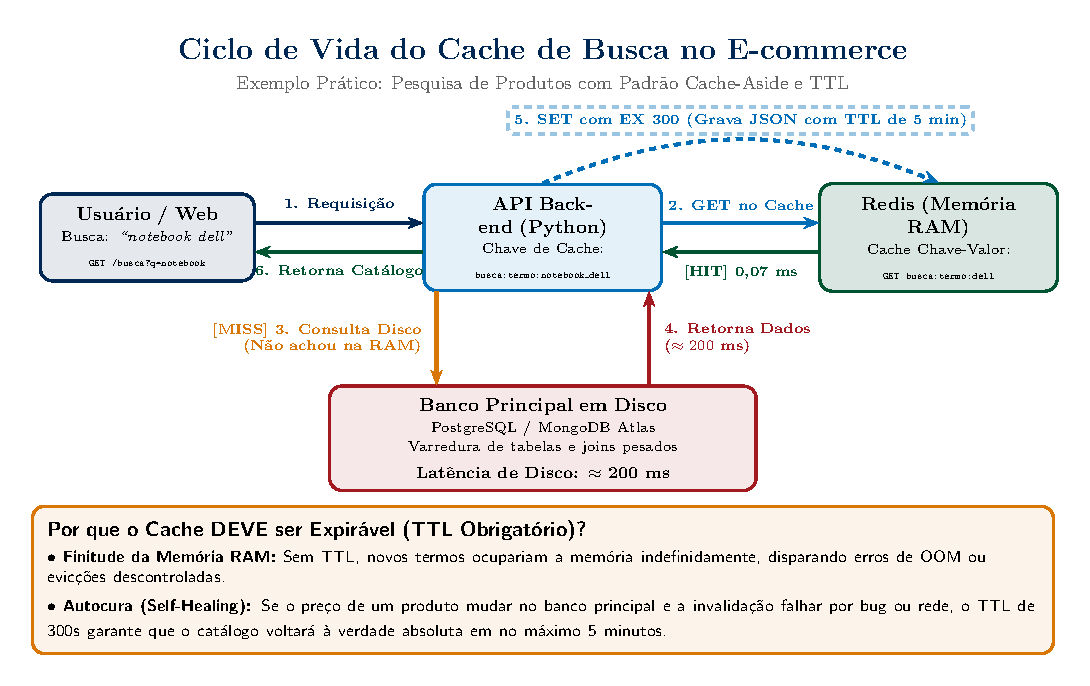
\includegraphics[width=0.90\textwidth,height=0.74\textheight,keepaspectratio]{figuras/fig_ciclo_cache_busca.pdf}
\end{frame}

% ------------------------------------------------------------------------------
\begin{frame}[fragile]{SET com Expiração Temporal (EX e PX)}
  \begin{columns}[T]
    \begin{column}{0.48\textwidth}
      \alert{Expiração Temporal (TTL)}\par
      \itemseps[topsepi=1mm,itemsepi=1.5mm,labelsep=2mm,leftmargini=4mm]
      \small
      \begin{itemize}
        \item O parâmetro \texttt{EX} define a expiração em segundos inteiros.
        \item O parâmetro \texttt{PX} define a expiração em milissegundos.
        \item Evita acúmulo descontrolado de dados obsoletos na memória RAM.
      \end{itemize}
    \end{column}
    \begin{column}{0.50\textwidth}
      \alert{Comandos no redis-cli}\par
      \begin{lstlisting}[language=bash]
# Gravar catalogo com TTL de 300s (5 min):
127.0.0.1:6379> SET busca:dell "[{id:1}]" EX 300
OK

# Consultar TTL restante em segundos:
127.0.0.1:6379> TTL busca:dell
(integer) 298

# Gravar chave com PX (2500 ms):
127.0.0.1:6379> SET ping:host "10.0.0.1" PX 2500
OK
      \end{lstlisting}
    \end{column}
  \end{columns}
\end{frame}

% ------------------------------------------------------------------------------
\begin{frame}[fragile]{SET com Trava Distribuída (Lock NX)}
  \begin{columns}[T]
    \begin{column}{0.48\textwidth}
      \alert{Exclusão Mútua Atômica}\par
      \itemseps[topsepi=1mm,itemsepi=1.5mm,labelsep=2mm,leftmargini=4mm]
      \small
      \begin{itemize}
        \item O modificador \texttt{NX} grava \textbf{apenas se a chave não existir}.
        \item Se a chave já existir, a gravação falha e devolve \texttt{(nil)}.
        \item \textbf{Caso Real:} Trava de concorrência para reservar a última unidade de um estoque.
      \end{itemize}
    \end{column}
    \begin{column}{0.50\textwidth}
      \alert{Comandos no redis-cli}\par
      \begin{lstlisting}[language=bash]
# Worker A adquire a trava por 15s:
127.0.0.1:6379> SET lock:prod:101 "wA" NX EX 15
OK

# Worker B tenta simultaneamente:
127.0.0.1:6379> SET lock:prod:101 "wB" NX EX 15
(nil)  # Bloqueado com sucesso!

# Liberacao manual da trava:
127.0.0.1:6379> DEL lock:prod:101
(integer) 1
      \end{lstlisting}
    \end{column}
  \end{columns}
\end{frame}

% ------------------------------------------------------------------------------
\begin{frame}[fragile]{SET Condicional (XX) e Preservação de TTL (KEEPTTL)}
  \begin{columns}[T]
    \begin{column}{0.48\textwidth}
      \alert{Atualização Estrita e TTL}\par
      \itemseps[topsepi=1mm,itemsepi=1.5mm,labelsep=2mm,leftmargini=4mm]
      \small
      \begin{itemize}
        \item \texttt{XX}: Grava \textbf{apenas se a chave já existir} (útil para atualizar status sem criar lixo).
        \item \texttt{KEEPTTL}: Atualiza o conteúdo da chave preservando a contagem de tempo restante.
      \end{itemize}
    \end{column}
    \begin{column}{0.50\textwidth}
      \alert{Comandos no redis-cli}\par
      \begin{lstlisting}[language=bash]
# Tentar atualizar chave inexistente:
127.0.0.1:6379> SET status:servico "on" XX
(nil)  # Nao cria chave nova

# Criar sessao com TTL de 60s:
127.0.0.1:6379> SET sessao:u1 "token_v1" EX 60
OK

# Atualizar valor mantendo o tempo:
127.0.0.1:6379> SET sessao:u1 "token_v2" KEEPTTL
OK  # O relogio regressivo nao zera!
      \end{lstlisting}
    \end{column}
  \end{columns}
\end{frame}

% ------------------------------------------------------------------------------
\begin{frame}[fragile]{SET com Troca Atômica (GET) e Lotes (MSET)}
  \begin{columns}[T]
    \begin{column}{0.48\textwidth}
      \alert{Substituição e Multi-Escrita}\par
      \itemseps[topsepi=1mm,itemsepi=1.5mm,labelsep=2mm,leftmargini=4mm]
      \small
      \begin{itemize}
        \item \texttt{SET ... GET}: Atualiza o valor e devolve o valor anterior atomicamente.
        \item \texttt{MSET}: Grava múltiplas chaves e valores em um único pacote TCP.
        \item Evita múltiplas viagens de ida e volta (RTT).
      \end{itemize}
    \end{column}
    \begin{column}{0.50\textwidth}
      \alert{Comandos no redis-cli}\par
      \begin{lstlisting}[language=bash]
# Substituir valor e receber o antigo:
127.0.0.1:6379> SET contagem:vendas 100 GET
"85"  # Retornou o valor anterior!

# Gravar varias moedas em 1 RTT:
127.0.0.1:6379> MSET usd 5.45 eur 5.95 btc 345k
OK

# Leitura conjunta imediata:
127.0.0.1:6379> MGET usd eur
1) "5.45"  2) "5.95"
      \end{lstlisting}
    \end{column}
  \end{columns}
\end{frame}

% ------------------------------------------------------------------------------
\begin{frame}[fragile]{GET Simples e em Lote (MGET)}
  \begin{columns}[T]
    \begin{column}{0.48\textwidth}
      \alert{Recuperação de Alta Velocidade}\par
      \itemseps[topsepi=1mm,itemsepi=1.5mm,labelsep=2mm,leftmargini=4mm]
      \small
      \begin{itemize}
        \item \texttt{GET}: Recupera uma única chave em $\mathcal{O}(1)$.
        \item \texttt{MGET}: Recupera múltiplas chaves de forma atômica.
        \item Chaves inexistentes retornam \texttt{(nil)} sem interromper a consulta das demais.
      \end{itemize}
    \end{column}
    \begin{column}{0.50\textwidth}
      \alert{Comandos no redis-cli}\par
      \begin{lstlisting}[language=bash]
# Leitura simples de termo cacheado:
127.0.0.1:6379> GET busca:dell
"[{id:1}]"

# Consulta de multiplas chaves:
127.0.0.1:6379> MGET usd eur chave_inexistente
1) "5.45"
2) "5.95"
3) (nil)
      \end{lstlisting}
    \end{column}
  \end{columns}
\end{frame}

% ------------------------------------------------------------------------------
\begin{frame}[fragile]{GETDEL: Consumo Atômico de Tokens de Uso Único}
  \begin{columns}[T]
    \begin{column}{0.48\textwidth}
      \alert{Leitura e Destruição em $\mathcal{O}(1)$}\par
      \itemseps[topsepi=1mm,itemsepi=1.5mm,labelsep=2mm,leftmargini=4mm]
      \small
      \begin{itemize}
        \item Lê o valor e \textbf{remove a chave atomicamente} em uma única operação.
        \item Elimina vulnerabilidade de reutilização concorrente (*double spending*).
        \item \textbf{Casos Reais:} Cobrança PIX, tokens de redefinição de senha e ingressos.
      \end{itemize}
    \end{column}
    \begin{column}{0.50\textwidth}
      \alert{Comandos no redis-cli}\par
      \begin{lstlisting}[language=bash]
# Gerar token PIX de 60 segundos:
127.0.0.1:6379> SET token:pix:99 "R$500" EX 60
OK

# Consumir e apagar atomicamente:
127.0.0.1:6379> GETDEL token:pix:99
"R$500"

# Segunda tentativa de leitura:
127.0.0.1:6379> GET token:pix:99
(nil)  # Ja consumido e destruido!
      \end{lstlisting}
    \end{column}
  \end{columns}
\end{frame}

% ------------------------------------------------------------------------------
\begin{frame}[fragile]{GETEX: Renovação Deslizante de Sessão}
  \begin{columns}[T]
    \begin{column}{0.48\textwidth}
      \alert{Extensão de Vida na Leitura}\par
      \itemseps[topsepi=1mm,itemsepi=1.5mm,labelsep=2mm,leftmargini=4mm]
      \small
      \begin{itemize}
        \item \texttt{GETEX}: Lê o dado e atualiza o seu TTL no mesmo instante.
        \item \textbf{Sessão Deslizante:} Enquanto o usuário navega na aplicação, a expiração é postergada sem comandos adicionais de escrita.
      \end{itemize}
    \end{column}
    \begin{column}{0.50\textwidth}
      \alert{Comandos no redis-cli}\par
      \begin{lstlisting}[language=bash]
# Sessao com TTL de 30s:
127.0.0.1:6379> SET sessao:u42 "jwt_token" EX 30
OK

# Ler e estender para 1800s (30m):
127.0.0.1:6379> GETEX sessao:u42 EX 1800
"jwt_token"

# Verificar novo tempo de expiracao:
127.0.0.1:6379> TTL sessao:u42
(integer) 1799
      \end{lstlisting}
    \end{column}
  \end{columns}
\end{frame}

% ------------------------------------------------------------------------------
\begin{frame}[fragile]{Inspeção de Strings (GETRANGE e STRLEN)}
  \begin{columns}[T]
    \begin{column}{0.48\textwidth}
      \alert{Substrings e Tamanho em Bytes}\par
      \itemseps[topsepi=1mm,itemsepi=1.5mm,labelsep=2mm,leftmargini=4mm]
      \small
      \begin{itemize}
        \item \texttt{GETRANGE}: Extrai intervalo de caracteres usando offsets de início e fim.
        \item \texttt{STRLEN}: Retorna o tamanho exato da string armazenada em bytes.
        \item Execução instantânea em memória.
      \end{itemize}
    \end{column}
    \begin{column}{0.50\textwidth}
      \alert{Comandos no redis-cli}\par
      \begin{lstlisting}[language=bash]
# Gravar mensagem textual:
127.0.0.1:6379> SET msg "IFCE Campus Taua"
OK

# Obter substring pelo intervalo [5, 10]:
127.0.0.1:6379> GETRANGE msg 5 10
"Campus"

# Medir comprimento em bytes:
127.0.0.1:6379> STRLEN msg
(integer) 16
      \end{lstlisting}
    \end{column}
  \end{columns}
\end{frame}

\changecolours{ScoutGreen}
\section{A Importância do Cache, Expiração e Práticas de Atualização}

% ------------------------------------------------------------------------------
\twocolframe[title={Por que o Cache DEVE ser Expirável (TTL)?},leftcol=7cm,rightcol=7cm]{%
  \alert{1. A Finitude Física da Memória RAM}\par
  \itemseps[topsepi=2mm,itemsepi=3mm,labelsep=2mm,leftmargini=4mm]
  \begin{itemize}
    \item A memória RAM custa significativamente mais por gigabyte que discos NVMe.
    \item Se gravarmos todas as buscas e consultas no Redis sem expiração, a RAM esgotará rapidamente.
    \item \textbf{Políticas de Evicção:} Quando atinge o \texttt{maxmemory}, o Redis descarta chaves via algoritmos LRU (\textit{Least Recently Used}) ou LFU (\textit{Least Frequently Used}).
  \end{itemize}
}{%
  \alert{2. Autocura Contra Dados Obsoletos}\par
  \itemseps[topsepi=2mm,itemsepi=3mm,labelsep=2mm,leftmargini=4mm]
  \begin{itemize}
    \item Em arquiteturas distribuídas, sincronizações podem falhar por timeout de rede ou concorrência.
    \item \textbf{Self-Healing:} Um TTL bem calibrado (ex: 60s a 300s) atua como rede de segurança.
    \item Mesmo que a invalidação ativa falhe, a chave expira e a próxima consulta busca a verdade atualizada na fonte primária.
  \end{itemize}
}

% ------------------------------------------------------------------------------
\begin{frame}{Padrões de Atualização de Cache e Sincronização}
  \centering
  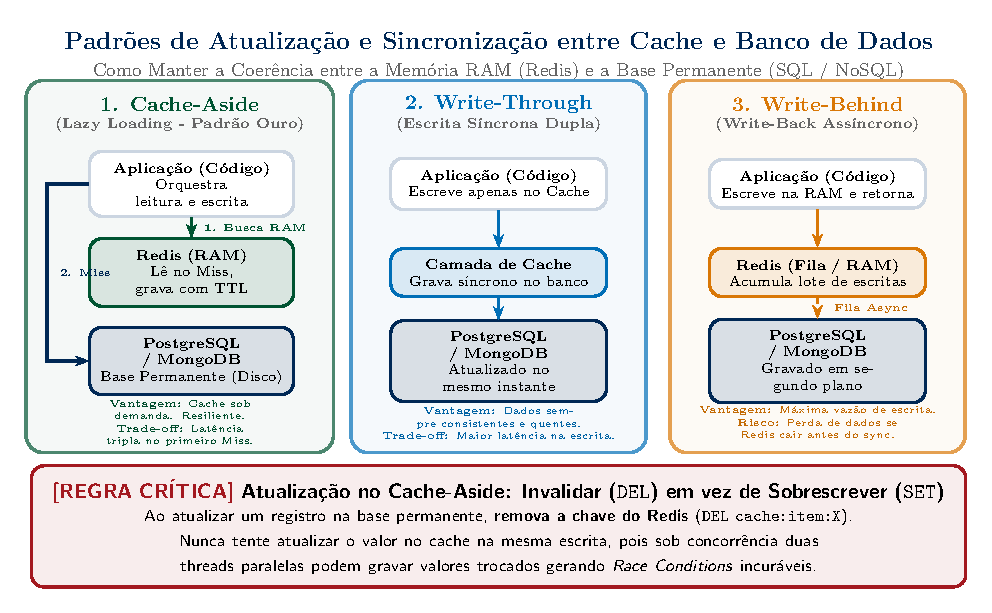
\includegraphics[width=0.90\textwidth,height=0.74\textheight,keepaspectratio]{figuras/fig_padroes_atualizacao.pdf}
\end{frame}

% ------------------------------------------------------------------------------
\twocolframe[title={Invalidação no Cache-Aside: O Risco de Race Conditions},leftcol=7cm,rightcol=7cm]{%
  \alert{O Erro Comum de Iniciante}\par
  \itemseps[topsepi=2mm,itemsepi=3mm,labelsep=2mm,leftmargini=4mm]
  \begin{itemize}
    \item Ao atualizar um produto no banco relacional, tentar atualizar o valor diretamente no Redis via \texttt{SET}.
    \item \textbf{Cenário de Desastre:} Sob alta concorrência, a Requisição 1 atualiza o SQL e depois a Requisição 2 atualiza o SQL.
    \item Porém, pela rede, o \texttt{SET} da Requisição 1 chega no Redis \textbf{depois} do \texttt{SET} da Requisição 2!
  \end{itemize}
}{%
  \alert{A Consequência Grave}\par
  \itemseps[topsepi=2mm,itemsepi=3mm,labelsep=2mm,leftmargini=4mm]
  \begin{itemize}
    \item O banco relacional permanente fica com o valor novo (da Requisição 2).
    \item O Redis fica com o valor velho (da Requisição 1) gravado para sempre!
    \item O cache torna-se inconsistente com a verdade do sistema.
  \end{itemize}
}

% ------------------------------------------------------------------------------
\begin{frame}[fragile]{Solução: A Regra de Ouro da Invalidação (DEL)}
  \begin{columns}[T]
    \begin{column}{0.48\textwidth}
      \alert{Invalidação Limpa e Segura}\par
      \itemseps[topsepi=1mm,itemsepi=1.5mm,labelsep=2mm,leftmargini=4mm]
      \small
      \begin{itemize}
        \item Ao alterar o banco permanente, \textbf{apenas delete a chave do Redis (\texttt{DEL})}.
        \item Não tente adivinhar o valor do cache na mesma escrita.
        \item A próxima leitura disparará \textit{Cache Miss}, recarregando a verdade da base SQL com novo TTL.
      \end{itemize}
    \end{column}
    \begin{column}{0.50\textwidth}
      \alert{Fluxo Seguro no Terminal}\par
      \begin{lstlisting}[language=bash]
# 1. Atualizar registro no banco SQL:
# UPDATE produtos SET preco=3599 WHERE id=101;

# 2. Invalidar imediatamente no Redis:
127.0.0.1:6379> DEL busca:item:101
(integer) 1

# 3. Proxima leitura busca no SQL e repovoa:
127.0.0.1:6379> SET busca:item:101 "3599" EX 300
OK
      \end{lstlisting}
    \end{column}
  \end{columns}
\end{frame}

% ------------------------------------------------------------------------------
\begin{frame}[fragile]{Políticas de Evicção de Memória sob Sobrecarga}
  \begin{columns}[T]
    \begin{column}{0.48\textwidth}
      \alert{Algoritmos no Limite de RAM}\par
      \itemseps[topsepi=1mm,itemsepi=1.5mm,labelsep=2mm,leftmargini=4mm]
      \small
      \begin{itemize}
        \item Ao atingir o limite \texttt{maxmemory}:
        \item \textbf{volatile-lru:} Descarta chaves com TTL menos acessadas recentemente (\textit{Recomendado para cache}).
        \item \textbf{allkeys-lru:} Descarta qualquer chave LRU.
        \item \textbf{noeviction:} Retorna erro em comandos de gravação quando a memória enche.
      \end{itemize}
    \end{column}
    \begin{column}{0.50\textwidth}
      \alert{Diretivas no redis.conf}\par
      \begin{lstlisting}[language=bash]
# Limite maximo de memoria para o Redis:
maxmemory 4gb

# Politica recomendada para camada de cache:
maxmemory-policy volatile-lru

# Inspecionar consumo de memoria no CLI:
127.0.0.1:6379> INFO memory
# used_memory_human:1.24M
      \end{lstlisting}
    \end{column}
  \end{columns}
\end{frame}

% ------------------------------------------------------------------------------
\begin{frame}{Comprovação Experimental: Benchmarking de Latência}
  \centering
  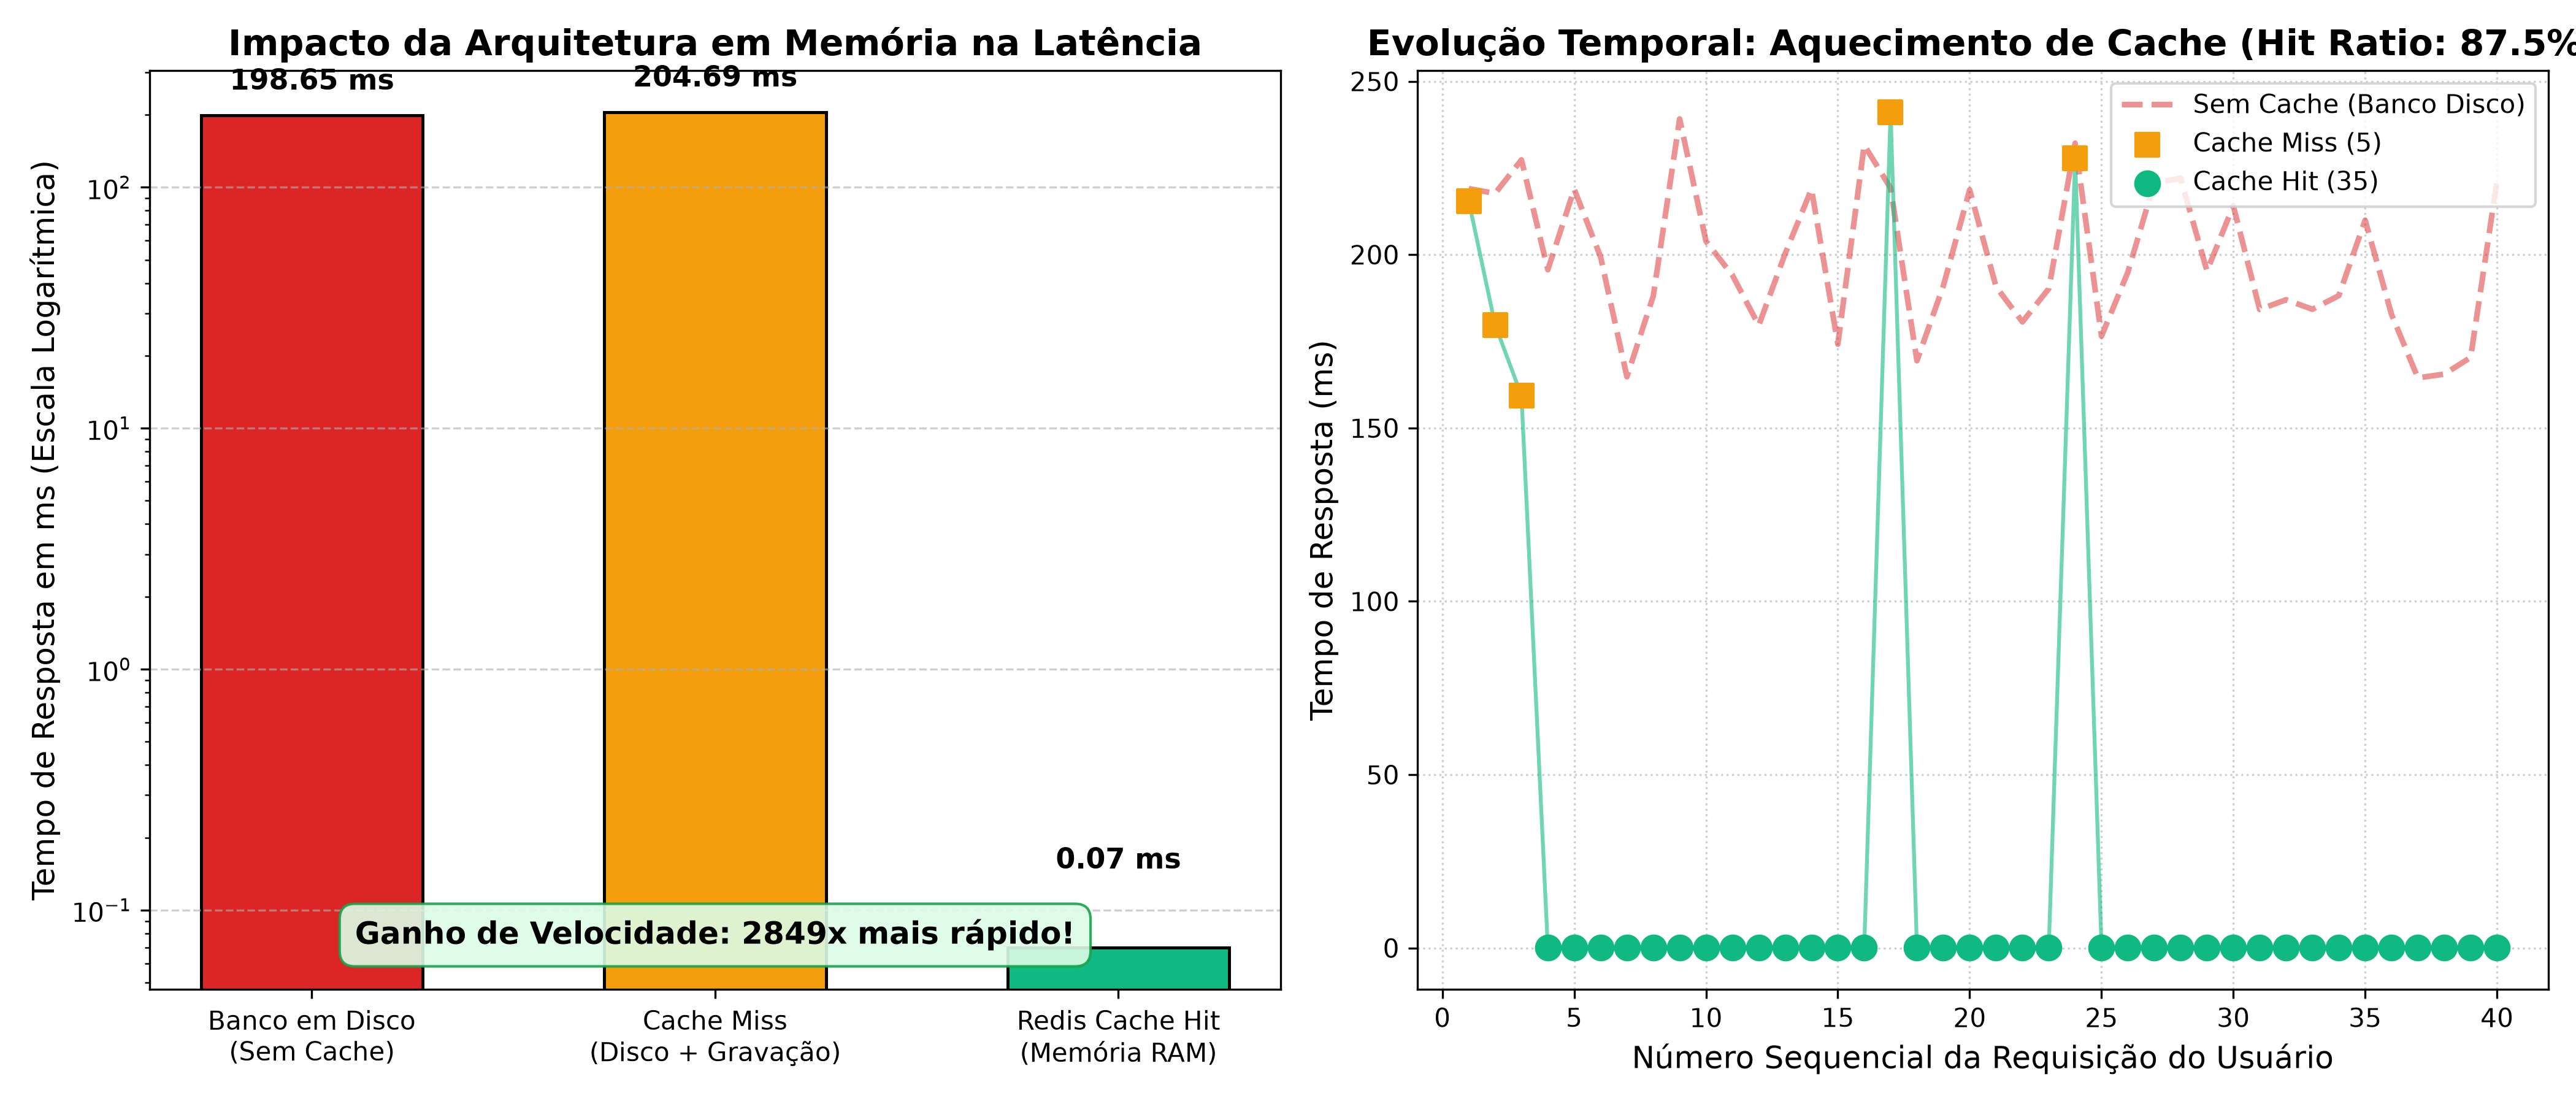
\includegraphics[width=0.88\textwidth,height=0.74\textheight,keepaspectratio]{figuras/grafico_latencia_busca.png}
\end{frame}

\changecolours{ScoutNavy}
\section{Estruturas Nativas e Modernização com Inteligência Artificial}

% ------------------------------------------------------------------------------
\begin{frame}{As 5 Estruturas de Dados Nativas do Redis}
  \centering
  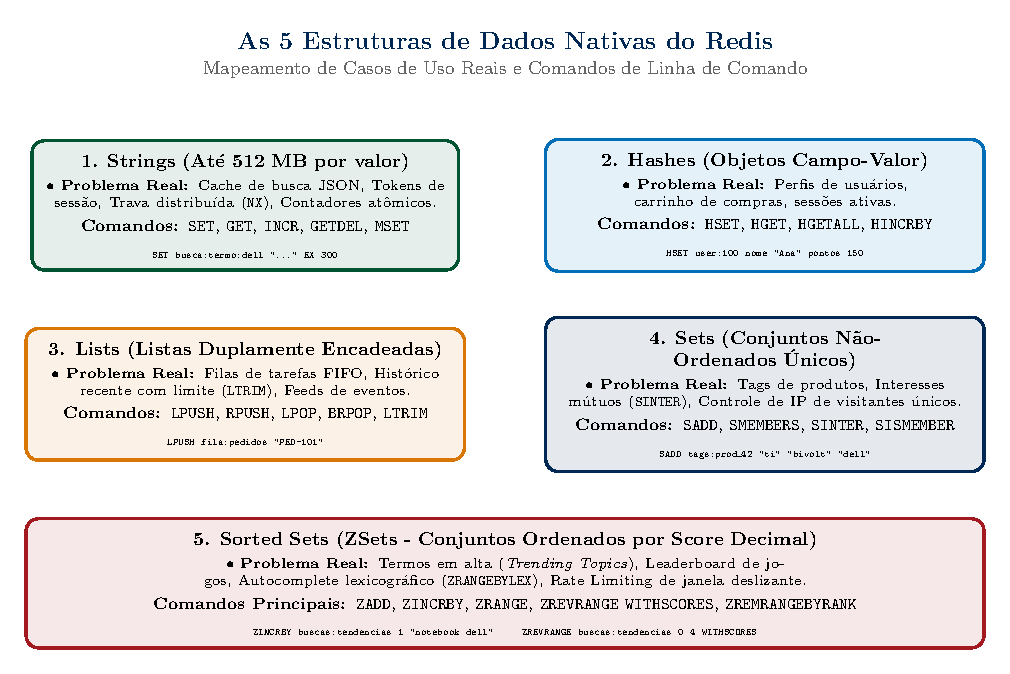
\includegraphics[width=0.90\textwidth,height=0.74\textheight,keepaspectratio]{figuras/fig_estruturas_redis.pdf}
\end{frame}

% ------------------------------------------------------------------------------
\begin{frame}[fragile]{Estrutura 2: Hashes (Objetos Campo-Valor)}
  \begin{columns}[T]
    \begin{column}{0.48\textwidth}
      \alert{Modelagem de Entidades}\par
      \itemseps[topsepi=1mm,itemsepi=1.5mm,labelsep=2mm,leftmargini=4mm]
      \small
      \begin{itemize}
        \item Mapeia dicionários campo-valor sob uma única chave.
        \item Permite alterar campos isolados sem trafegar o JSON todo.
        \item \textbf{Casos Reais:} Perfis de usuários, carrinhos e preferências.
      \end{itemize}
    \end{column}
    \begin{column}{0.50\textwidth}
      \alert{Comandos no redis-cli}\par
      \begin{lstlisting}[language=bash]
# Criar perfil de aluno com campos:
127.0.0.1:6379> HSET user:aluno:42 nome "Ana" pontos 80
(integer) 2

# Incrementar pontuacao atomicamente:
127.0.0.1:6379> HINCRBY user:aluno:42 pontos 20
(integer) 100

# Ler campo isolado em O(1):
127.0.0.1:6379> HGET user:aluno:42 pontos
"100"

# Recuperar todos os pares:
127.0.0.1:6379> HGETALL user:aluno:42
1) "nome"    2) "Ana"
3) "pontos"  4) "100"
      \end{lstlisting}
    \end{column}
  \end{columns}
\end{frame}

% ------------------------------------------------------------------------------
\begin{frame}[fragile]{Estrutura 3: Lists (Filas FIFO e Históricos)}
  \begin{columns}[T]
    \begin{column}{0.48\textwidth}
      \alert{Listas Duplamente Encadeadas}\par
      \itemseps[topsepi=1mm,itemsepi=1.5mm,labelsep=2mm,leftmargini=4mm]
      \small
      \begin{itemize}
        \item Inserção rápida nas pontas (\texttt{LPUSH} / \texttt{RPUSH}).
        \item \textbf{Capped Lists:} \texttt{LTRIM} mantém tamanho fixo.
        \item \textbf{Casos Reais:} Filas de tarefas FIFO e histórico de buscas recentes.
      \end{itemize}
    \end{column}
    \begin{column}{0.50\textwidth}
      \alert{Comandos no redis-cli}\par
      \begin{lstlisting}[language=bash]
# Adicionar buscas recentes:
127.0.0.1:6379> LPUSH hist:42 "python" "nosql" "redis"
(integer) 3

# Manter apenas as 2 mais recentes:
127.0.0.1:6379> LTRIM hist:42 0 1
OK

# Consultar historico podado:
127.0.0.1:6379> LRANGE hist:42 0 -1
1) "redis"  2) "nosql"

# Consumir da ponta oposta (FIFO):
127.0.0.1:6379> RPOP hist:42
"nosql"
      \end{lstlisting}
    \end{column}
  \end{columns}
\end{frame}

% ------------------------------------------------------------------------------
\begin{frame}[fragile]{Estrutura 4: Sets (Conjuntos Únicos e Álgebra)}
  \begin{columns}[T]
    \begin{column}{0.48\textwidth}
      \alert{Conjuntos Não-Ordenados Únicos}\par
      \itemseps[topsepi=1mm,itemsepi=1.5mm,labelsep=2mm,leftmargini=4mm]
      \small
      \begin{itemize}
        \item Garante unicidade de membros em $\mathcal{O}(1)$.
        \item Suporta álgebra de conjuntos: Interseção (\texttt{SINTER}), União (\texttt{SUNION}).
        \item \textbf{Casos Reais:} Tags de catálogo e visitantes únicos.
      \end{itemize}
    \end{column}
    \begin{column}{0.50\textwidth}
      \alert{Comandos no redis-cli}\par
      \begin{lstlisting}[language=bash]
# Cadastrar tags de dois produtos:
127.0.0.1:6379> SADD tags:prodA "ti" "bivolt" "dell"
(integer) 3
127.0.0.1:6379> SADD tags:prodB "eletro" "bivolt" "dell"
(integer) 3

# Testar pertinencia em O(1):
127.0.0.1:6379> SISMEMBER tags:prodA "dell"
(integer) 1

# Intersecao: Tags compartilhadas:
127.0.0.1:6379> SINTER tags:prodA tags:prodB
1) "dell"  2) "bivolt"
      \end{lstlisting}
    \end{column}
  \end{columns}
\end{frame}

% ------------------------------------------------------------------------------
\begin{frame}[fragile]{Estrutura 5: Sorted Sets (Rankings e Tendências)}
  \begin{columns}[T]
    \begin{column}{0.48\textwidth}
      \alert{Conjuntos Ordenados por Pontuação}\par
      \itemseps[topsepi=1mm,itemsepi=1.5mm,labelsep=2mm,leftmargini=4mm]
      \small
      \begin{itemize}
        \item Cada membro possui um \textbf{score numérico}.
        \item Mantém a coleção ordenada em memória via SkipList interna.
        \item \textbf{Casos Reais:} \textit{Trending Topics} de busca em tempo real e leaderboards.
      \end{itemize}
    \end{column}
    \begin{column}{0.50\textwidth}
      \alert{Comandos no redis-cli}\par
      \begin{lstlisting}[language=bash]
# Inicializar termos com volume de buscas:
127.0.0.1:6379> ZADD rank:buscas 100 "notebook" 150 "celular"
(integer) 2

# Incrementar busca em tempo real:
127.0.0.1:6379> ZINCRBY rank:buscas 85 "notebook"
"185"

# Top 2 mais buscados decrescente:
127.0.0.1:6379> ZREVRANGE rank:buscas 0 1 WITHSCORES
1) "notebook"  2) "185"
3) "celular"   4) "150"
      \end{lstlisting}
    \end{column}
  \end{columns}
\end{frame}

% ------------------------------------------------------------------------------
\begin{frame}{Modernização: Redis como Camada de Contexto para IA}
  \centering
  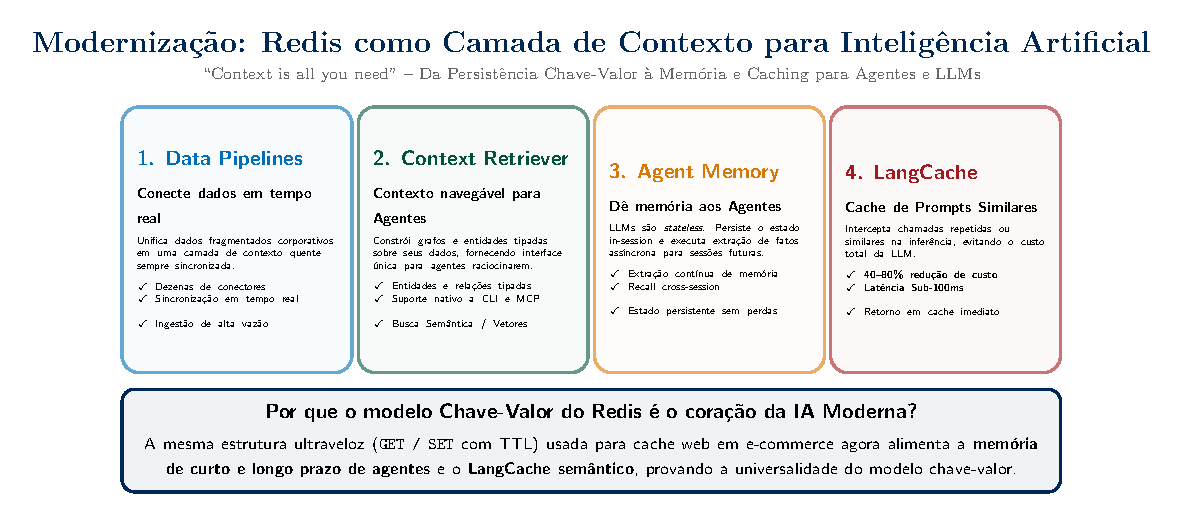
\includegraphics[width=0.90\textwidth,height=0.74\textheight,keepaspectratio]{figuras/fig_redis_ai_langcache.pdf}
\end{frame}

% ------------------------------------------------------------------------------
\twocolframe[title={Atividades Práticas e Próximos Passos},leftcol=7cm,rightcol=7cm]{%
  \alert{Laboratório Hands-On de Hoje}\par
  \itemseps[topsepi=2mm,itemsepi=3mm,labelsep=2mm,leftmargini=4mm]
  \begin{itemize}
    \item Executar o script de terminal \texttt{redis\_cli\_guia\_pratico.sh}.
    \item Praticar no terminal \texttt{redis-cli} as variações de \texttt{SET} (\texttt{NX}, \texttt{EX}, \texttt{KEEPTTL}) e \texttt{GET} (\texttt{GETDEL}, \texttt{MGET}).
    \item Testar a persistência disparando \texttt{BGSAVE} e inspecionando \texttt{LASTSAVE}.
    \item Rodar o script Python interativo \texttt{demonstracao\_aula04.py} e inspecionar os tempos de latência.
  \end{itemize}
}{%
  \alert{Conexão com a Aula 05}\par
  \itemseps[topsepi=2mm,itemsepi=3mm,labelsep=2mm,leftmargini=4mm]
  \begin{itemize}
    \item Na próxima aula (\textbf{Aula 05 - 20/10/2026}), aprofundaremos as \textbf{Estratégias Avançadas de Caching, Controle de Sessões e Filas de Mensagens (Streams)}.
    \item Resolver a lista de exercícios práticos da Aula 04 disponível no portal web da disciplina.
    \item O código e slides estão disponíveis no repositório oficial da turma.
  \end{itemize}
}


% ------------------------------------------------------------------------------
% Encerramento
% ------------------------------------------------------------------------------
\changecolours[inverse]{ScoutGreen}
\begin{frame}[plain]
  \vspace{2cm}
  \centering
  {\Huge \textbf{Dúvidas \& Discussão}}\par
  \vspace{0.8cm}
  {\large IFCE Campus Tauá -- ADS16}\par
  \vspace{0.3cm}
  {\small reginaldo.fernandes@ifce.edu.br}
\end{frame}

\end{document}
